\documentclass{../../../oss-ap12ibhl-print}
\usepackage{bm}

\begin{document}
\genheader

\gentitle{1}{KINEMATICS}

\textbf{Questions 1--2}

A ball of mass \SI{.5}{\kilo\gram} is launched horizontally from the top of a
cliff \SI{80}{\metre} high with a speed of \SI{20}{\metre\per\second} at time
$t=0$.
\begin{center}
  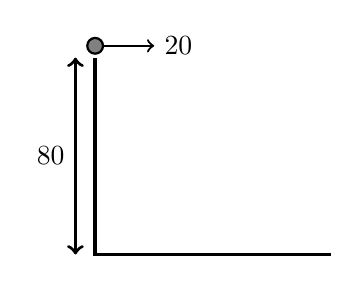
\begin{tikzpicture}[scale=.5]
    \draw[very thick](0,5)--(0,0)--(6,0);
    \draw[<->,very thick](-.5,0)--(-.5,5) node[midway,left]{\SI{80}{\metre}};
    \draw[thick,->](0,5.3)--(1.5,5.3)
    node[pos=1,right]{\SI{20}{\metre\per\second}};
    \draw[thick,fill=gray](0,5.3) circle(.2);
  \end{tikzpicture}
\end{center}
  
\begin{questions}
  \question The horizontal distance $x$ traveled by the ball before striking the
  ground is

  \begin{oneparchoices}
    \choice\SI{20}{\metre}\hspace{.4in}
    \choice\SI{40}{\metre}\hspace{.4in}
    \choice\SI{80}{\metre}\hspace{.4in} 
    \choice\SI{160}{\metre}\hspace{.4in}
    \choice\SI{320}{\metre}
  \end{oneparchoices}

  \question The speed of the ball just before striking the ground is

  \begin{oneparchoices}
    \choice\SI{4}{\metre\per\second}\hspace{.3in}
    \choice\SI{14}{\metre\per\second}\hspace{.3in}
    \choice\SI{20}{\metre\per\second}\hspace{.3in}
    \choice\SI{44}{\metre\per\second}\hspace{.3in}
    \choice\SI{64}{\metre\per\second}
  \end{oneparchoices}
  
  \uplevel{\rule{\linewidth}{.6pt}}

  \question A space explorer throws a tool downward on a planet with an initial
  velocity of \SI{2}{\metre\per\second} from a height of \SI{6}{\metre}
  above the surface. The tool strikes the surface in a time of \SI{2}{\second}.
  The acceleration due to gravity on the planet is

  \begin{oneparchoices}
    \choice\SI{1}{\metre\per\second\squared}\hspace{.27in}
    \choice\SI{2}{\metre\per\second\squared}\hspace{.27in}
    \choice\SI{3}{\metre\per\second\squared}\hspace{.27in}
    \choice\SI{4}{\metre\per\second\squared}\hspace{.27in}
    \choice\SI{10}{\metre\per\second\squared}
  \end{oneparchoices}
  
  \uplevel{\rule{\linewidth}{.6pt}}

  \uplevel{
    \textbf{Questions \ref{q:sprinter1}--\ref{q:sprinter2}}
  
    A sprinter starting from rest runs a \SI{100}{\metre} race on a straight
    track. The sprinter covers the first \SI{10}{\metre} with a constant
    acceleration in 2 seconds. The sprinter runs the remaining \SI{90}{\metre}
    with the same velocity he had at the end of \SI{2}{\second}.
  }
  
  \question The sprinter's velocity at the end of the first \SI{2}{\second} is

  \begin{oneparchoices}
    \choice\SI{5 }{\metre\per\second}\hspace{.27in}
    \choice\SI{10}{\metre\per\second}\hspace{.27in}
    \choice\SI{20}{\metre\per\second}\hspace{.27in}
    \choice\SI{40}{\metre\per\second}\hspace{.27in}
    \choice\SI{60}{\metre\per\second}
  \end{oneparchoices}
  \label{q:sprinter1}
  
  \question The total time it takes for the sprinter to run the full
  \SI{100}{\metre} is
  
  \begin{oneparchoices}
    \choice\SI{2}{\second}\hspace{.5in}
    \choice\SI{9}{\second}\hspace{.5in}
    \choice\SI{10}{\second}\hspace{.5in}
    \choice\SI{11}{\second}\hspace{.5in}
    \choice\SI{12}{\second}
  \end{oneparchoices}
  \label{q:sprinter2}
  
  \uplevel{\rule{\linewidth}{.6pt}}
  
  \question A block of mass \SI{2}{\kilo\gram} is attached to a string that is
  wrapped around a pulley of negligible mass and allowed to descend from rest
  a vertical distance of \SI{1.2}{\metre} in a time of \SI{1.5}{\second}. The
  acceleration of the block is most nearly

  \begin{minipage}{.28\linewidth}
    \pic{.8}{block-pulley}
    % I CAN PROBABLY DO WITH A BETTER DIAGRAM HERE!
  \end{minipage}
  \begin{minipage}{.3\linewidth}
    \begin{choices}
      \choice\SI{.2}{\metre\per\second\squared}
      \choice\SI{.6}{\metre\per\second\squared}
      \choice\SI{1.1}{\metre\per\second\squared}
      \choice\SI{1.4}{\metre\per\second\squared}
      \choice\SI{1.5}{\metre\per\second\squared}
    \end{choices}
  \end{minipage}
  \newpage
  
  \question A golf ball is hit from level ground and has a horizontal range of
  \SI{100}{\metre}. The ball leaves the golf club at an angle of \ang{60} to
  the level ground. At what other angle(s) can the ball be struck at the same
  initial velocity and still have a range of \SI{100}{\metre}?

  \begin{minipage}{.38\linewidth}
    \pic{.85}{golf-ball}
  \end{minipage}
  \begin{minipage}{.61\linewidth}
    \begin{choices}
      \choice\ang{30}
      \choice\ang{20} and \ang{80}
      \choice\ang{10} and \ang{120}
      \choice\ang{45} and \ang{135}
      \choice There is no other angle other than \ang{60} in which the ball
      will have a range of \SI{100}{\metre}.
    \end{choices}
  \end{minipage}

  \uplevel{\rule{\linewidth}{.6pt}}
  
  \question A small airplane can fly at \SI{200}{\kilo\metre\per\hour} with no
  wind. The pilot of the plane would like to fly to a destination
  \SI{100}{\kilo\metre} due north of his present position, but there is a
  crosswind of \SI{50}{\kilo\metre\per\hour} east. How much time is required
  for the plane to fly north to its destination?
  \begin{choices}
    \choice less than \SI{1/2}{\hour}
    \choice \SI{1/2}{\hour}
    \choice more than \SI{1/2}{\hour}
    \choice \SI{1}{\hour}
    \choice more than \SI{1}{\hour}
  \end{choices}

  \uplevel{\rule{\linewidth}{.6pt}}
  
  \uplevel{
    \textbf{Questions \ref{q:particle1}--\ref{q:particle2}}
    
    A particle moves on a horizontal surface with a constant acceleration of
    \SI{6}{\metre\per\second\squared} in the $x$-direction and
    \SI{4}{\metre\per\second\squared} in the $y$-direction. The initial
    velocity of the particle is \SI{3}{\metre\per\second} in the $x$-direction.
  }

  \question The speed of the particle after \SI{4}{\second} is

  \begin{oneparchoices}
    \choice\SI{16}{\metre\per\second}\hspace{.27in}
    \choice\SI{27}{\metre\per\second}\hspace{.27in}
    \choice\SI{31}{\metre\per\second}\hspace{.27in}
    \choice\SI{44}{\metre\per\second}\hspace{.27in}
    \choice\SI{985}{\metre\per\second}
  \end{oneparchoices}
  \label{q:particle1}
    
  \question The displacement of the particle from its initial position is

  \begin{oneparchoices}
    \choice\SI{16}{\metre}\hspace{.4in}
    \choice\SI{32}{\metre}\hspace{.4in}
    \choice\SI{60}{\metre}\hspace{.4in}
    \choice\SI{68}{\metre}\hspace{.4in}
    \choice\SI{92}{\metre}
  \end{oneparchoices}
  \label{q:particle2}

  \uplevel{\rule{\linewidth}{.6pt}}
  
  \question A small ball is launched with a speed of \SI{8}{\metre\per\second}
  at an angle of \ang{30} from the horizontal. A cup is hung so that it is in
  position to catch the ball when it reaches its maximum height. How far above
  the floor should the cup be hung to catch the ball?

  \begin{minipage}{.35\linewidth}
    \pic{.8}{cup}
  \end{minipage}
  \begin{minipage}{.4\linewidth}
    \begin{choices}
      \choice\SI{2.4}{\metre}
      \choice\SI{1.6}{\metre}
      \choice\SI{1.}{\metre}
      \choice\SI{.8}{\metre}
      \choice\SI{.4}{\metre}
    \end{choices}
  \end{minipage}

  \uplevel{
    \rule{\linewidth}{.6pt}
    
    \textbf{Questions \ref{q:graph1}--\ref{q:graph2}}

    The graph shown below represents the velocity vs.\ time graphs for two cars,
    $P$ and $Q$. Car $P$ begins with a speed $v_P$, and Car $Q$ begins with a
    speed $v_Q$ which is twice the velocity of Car $P$, that is, $v_Q=2v_P$.
    \begin{center}
      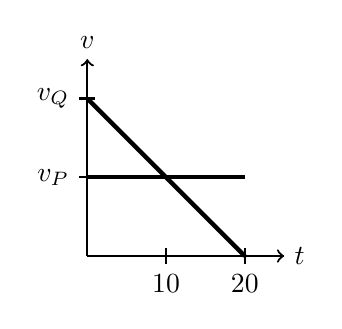
\begin{tikzpicture}[scale=.5]
        \draw[thick,->](0,0)--(5,0) node[right]{$t$};
        \draw[thick,->](0,0)--(0,5) node[above]{$v$};
        \draw[ultra thick](0,4)--(4,0);
        \draw[ultra thick](0,2)--(4,2);
        \draw[thick](2,.2)--(2,-.2) node[below]{10};
        \draw[thick](4,.2)--(4,-.2) node[below]{20};
        \draw[thick](.2,4)--(-.2,4) node[left]{$v_Q$};
        \draw[thick](.2,2)--(-.2,2) node[left]{$v_P$};
      \end{tikzpicture}
    \end{center}
  }

  \question\vspace{-.15in}Which of the following is true at a time of
  \SI{10}{\second}?
  \begin{choices}
    \choice The cars occupy the same position.
    \choice Car $P$ is at rest.
    \choice $v_Q>v_P$
    \choice $v_P>v_Q$
    \choice Car $Q$ is ahead of Car $P$.
  \end{choices}
  \label{q:graph1}
    
  \question Which of the following is true at a time of \SI{20}{\second}?
  \begin{choices}
    \choice The cars occupy the same position.
    \choice Car $P$ is at rest.
    \choice $v_Q>v_P$
    \choice $a_P=a_Q$
    \choice Car $P$ is ahead of Car $Q$.
  \end{choices}
  \label{q:graph2}

  \uplevel{\rule{\linewidth}{.6pt}}
  
  \question The velocity vs.\ time graph below represents the motion of a
  bicycle rider. The displacement of the rider between $0$ and \SI{4}{\hour} is

  \begin{minipage}{.4\linewidth}
    \pic{.8}{bikerider}
  \end{minipage}
  \begin{minipage}{.4\linewidth}
    \begin{choices}
      \choice +\SI{10}{\kilo\metre}
      \choice +\SI{20}{\kilo\metre}
      \choice +\SI{30}{\kilo\metre}
      \choice +\SI{40}{\kilo\metre}
      \choice \SI{-10}{\kilo\metre}
    \end{choices}
  \end{minipage}
  
  \uplevel{\rule{\linewidth}{.6pt}}
  
  \question A car is initially moving with a positive velocity of
  \SI{20}{\metre\per\second} when it passes the origin at time $t=0$. The car
  continues to move at \SI{20}{\metre\per\second} between $t=0$ and
  $t=\SI{2}{\second}$. At $t=\SI{2}{\second}$, the driver presses the brake,
  giving the car an acceleration of \SI{-4}{\metre\per\second\squared}. The
  displacement of the car at $t=\SI{6}{\second}$ is

  \begin{oneparchoices}
    \choice\SI{40}{\metre}\hspace{.28in}
    \choice\SI{32}{\metre}\hspace{.28in}
    \choice\SI{48}{\metre}\hspace{.28in}
    \choice\SI{64}{\metre}\hspace{.28in}
    \choice\SI{88}{\metre}
  \end{oneparchoices}

  \uplevel{\rule{\linewidth}{.6pt}}
  
  \question A \SI{600}{\kilo\gram} car accelerates uniformly from rest. After
  \SI{4}{\second}, it reaches a speed of \SI{24}{\metre\per\second}. During
  the \SI{4}{\second}, the car has traveled a distance of

  \begin{oneparchoices}
    \choice\SI{12}{\metre}\hspace{.28in}
    \choice\SI{24}{\metre}\hspace{.28in}
    \choice\SI{36}{\metre}\hspace{.28in}
    \choice\SI{48}{\metre}\hspace{.28in}
    \choice\SI{96}{\metre}
  \end{oneparchoices}
  \newpage
  
  \question Two velocity vectors $v_1$ and $v_2$ each have a magnitude of
  \SI{10}{\metre\per\second}. Graph 1 shows the velocity $v_1$ at
  $t=\SI0{\second}$, and then the same object has a velocity $v_2$ at
  $t=\SI{2}{\second}$, shown in Graph 2. Which of the following vectors
  represents the average acceleration vector that causes the object's velocity
  to change from $v_1$ to $v_2$ ?
  \begin{center}
    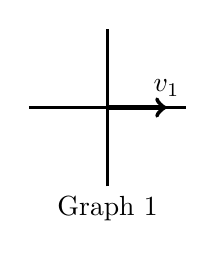
\begin{tikzpicture}[scale=.5]
      \draw[thick](-2,0)--(2,0);
      \draw[thick](0,-2)--(0,2) node[pos=0,below]{Graph 1};
      \draw[ultra thick,->](0,0)--(1.5,0) node[above]{$v_1$};
    \end{tikzpicture}
    \hspace{.2in}
    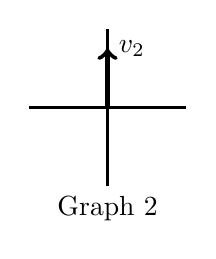
\begin{tikzpicture}[scale=.5]
      \draw[thick](-2,0)--(2,0);
      \draw[thick](0,-2)--(0,2) node[pos=0,below]{Graph 2};
      \draw[ultra thick,->](0,0)--(0,1.5) node[right]{$v_2$};
    \end{tikzpicture}
  \end{center}
  \begin{oneparchoices}
    \choice
    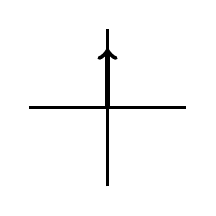
\begin{tikzpicture}[scale=.5]
      \draw[thick](-2,0)--(2,0);
      \draw[thick](0,-2)--(0,2);
      \draw[ultra thick,->](0,0)--(0,1.5);
    \end{tikzpicture}
    \choice
    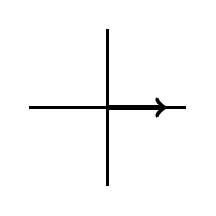
\begin{tikzpicture}[scale=.5]
      \draw[thick](-2,0)--(2,0);
      \draw[thick](0,-2)--(0,2);
      \draw[ultra thick,->](0,0)--(1.5,0);
    \end{tikzpicture}
    \choice
    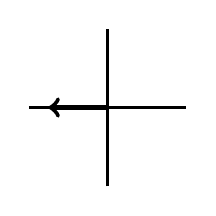
\begin{tikzpicture}[scale=.5]
      \draw[thick](-2,0)--(2,0);
      \draw[thick](0,-2)--(0,2);
      \draw[ultra thick,->](0,0)--(-1.5,0);
    \end{tikzpicture}
    \choice
    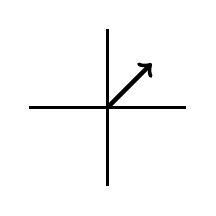
\begin{tikzpicture}[scale=.5]
      \draw[thick](-2,0)--(2,0);
      \draw[thick](0,-2)--(0,2);
      \draw[ultra thick,->](0,0)--(1.12,1.12);
      \end{tikzpicture}
    \choice
    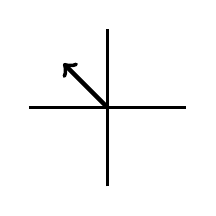
\begin{tikzpicture}[scale=.5]
      \draw[thick](-2,0)--(2,0);
      \draw[thick](0,-2)--(0,2);
      \draw[ultra thick,->](0,0)--(-1.12,1.12);
    \end{tikzpicture}
  \end{oneparchoices}

  \uplevel{\rule{\linewidth}{.6pt}}
  
  \question A toy dart gun fires a dart at an angle of \ang{45} to the
  horizontal and the dart reaches a maximum height of 1 meter. If the dart
  were fired straight up into the air along the vertical, the dart would
  reach a height of
  
  \begin{oneparchoices}
    \choice\SI{1}{\metre}\hspace{.4in}
    \choice\SI{2}{\metre}\hspace{.4in}
    \choice\SI{3}{\metre}\hspace{.4in}
    \choice\SI{4}{\metre}\hspace{.4in}
    \choice\SI{5}{\metre}
  \end{oneparchoices}

  \uplevel{\rule{\linewidth}{.6pt}}
  
  \question A ball is hit straight up into the air with an upward positive
  velocity. Wich of the following describes the velocity and acceleration
  of the ball at the instant it reaches the top of its flight?
  
  \begin{tabular}{lcc}
    & Velocity & Acceleration\\ \hline
    (A) & $0$ & $0$\\
    (B) & $0$ & $g$\\
    (C) & $2v_0$ & $g$\\
    (D) & $\dfrac12v_0$ & $0$\\
    (E) & $0$ & $\dfrac12g$
  \end{tabular}
  \uplevel{\rule{\linewidth}{.6pt}}
  
  \question The motion of an object is represented by the acceleration vs.\ time
  graph below. The object begins from rest. Which of the following statements
  is true about the motion of the object?

  \begin{minipage}{.3\linewidth}
    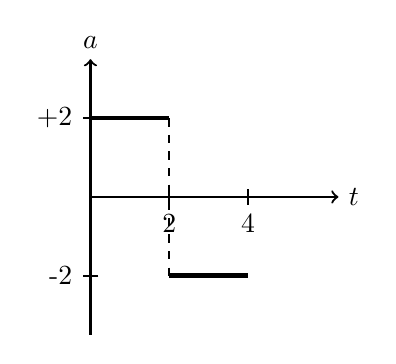
\begin{tikzpicture}[scale=.5]
      \draw[thick,->](0,0)--(6.3,0) node[right]{$t$};
      \draw[thick,->](0,-3.5)--(0,3.5) node[above]{$a$};
      \draw[ultra thick](0,2)--(2,2);
      \draw[ultra thick](2,-2)--(4,-2);
      \draw[dashed,thick](2,2)--(2,-2);
      \draw[thick](2,.2)--(2,-.2) node[below]{2};
      \draw[thick](4,.2)--(4,-.2) node[below]{4};
      \draw[thick](.2,2)--(-.2,2) node[left]{+2};
      \draw[thick](.2,-2)--(-.2,-2) node[left]{-2};
    \end{tikzpicture}
  \end{minipage}
  \begin{minipage}{.6\linewidth}
    \begin{choices}
      \choice The object returns to its original position.
      \choice The velocity of the object is zero at a time of \SI{2}{\second}.
      \choice The velocity of the object is zero at a time of \SI{4}{\second}.
      \choice The displacement of the object is zero at a time of
      \SI{4}{\second}.
      \choice The acceleration of the object is zero at a time of
      \SI{2}{\second}.
    \end{choices}
  \end{minipage}
  \newpage
  
  % THIS IS TAKEN FROM 2001 AP PHYSICS B EXAM, FREE-RESPONSE QUESTION #2
  \uplevel{
    \cpic{.6}{position-graph}
  }
  \question The vertical position of an elevator as a function of time is shown
  above.
  \begin{parts}
    \part On the grid below, graph the velocity of the elevator as a function of
    time.
    \cpic{.7}{velocity-graph}
    
    \part 
    \begin{subparts}
      \subpart Calculate the average acceleration for the time period
      $t=\SI{8}{\second}$ to $t=\SI{10}{\second}$.
      \subpart On the box below that represents the elevator, draw a vector to
      represent the direction of this average acceleration.
      \begin{center}
        \vspace{.5in}

        {\tikz \draw[thick](0,0) rectangle(1,1);}
        \vspace{.5in}
      \end{center}
    \end{subparts}
    
    \part Suppose that there is a passenger of mass \SI{70}{\kilo\gram} in the
    elevator. Calculate the apparent weight of the passenger at time
    $t=\SI{4}{\second}$.
  \end{parts}
  \newpage
  
  % TAKEN FROM 2001 AP PHYSICS B EXAM FREE-RESPONSE QUESTION 2
  \uplevel{
    \cpic{.7}{table1}
  }
  \question An incident ball $A$ of mass \SI{.10}{\kilo\gram} is sliding at
  \SI{1.4}{\metre\per\second} on the horizontal tabletop of negligible friction
  shown above. It makes a head-on collision with a target ball $B$ of mass
  \SI{.50}{\kilo\gram} at rest at the edge of the table. As a result of the
  collision, the incident ball rebounds, sliding backwards at
  \SI{.70}{\metre\per\second} immediately after the collision.
  \begin{parts}
    \part Calculate the speed of the \SI{.50}{\kilo\gram} target ball
    immediately after the collision.
    \uplevel{
      The tabletop is 1.20 m above a level, horizontal floor. The target ball is
      projected horizontally and initially strikes the floor at a horizontal
      displacement $d$ from the point of collision.
    }

    \part Calculate the horizontal displacement $d$.
  
    \uplevel{
      \cpic{.6}{table2}
      In another experiment on the same table, the target ball $B$ is replaced
      by target ball $C$ of mass 0.10 kg. The incident ball $A$ again slides at
      \SI{1.4}{\metre\per\second}, as shown above left, but this time makes a
      glancing collision with the target ball $C$ that is at rest at the edge of
      the table. The target ball $C$ strikes the floor at point $P$, which is
      at a horizontal displacement of \SI{.15}{\metre} from the point of the
      collision, and at a horizontal angle of \ang{30} from the $+x$-axis, as
      shown above right.
    }

    \part Calculate the speed $v$ of the target ball $C$ immediately after the
    collision.

    \part Calculate the $y$-component of incident ball $A$'s momentum
    immediately after the collision.
  \end{parts}
  \newpage


  
  % TAKEN FROM 2016 AP PHYSICS 1 FREE-RESPONSE QUESTION 3
  \uplevel{
    \centering
    \pic{.8}{ramp-down}
    
    \underline{Note:} Figure not drawn to scale.
  }
  
  \question (Suggested time 25 minutes) A long track, inclined at an angle
  $\theta$ to the horizontal, has small speed bumps on it. The bumps are evenly
  spaced a distance $d$ apart, as shown in the figure above. The track is
  actually much longer than shown, with over 100 bumps. A cart of mass $M$ is
  released from rest at the top of the track. A student notices that after
  reaching the 40th bump the cart's average speed between successive bumps no
  longer increases, reaching a maximum value $v_\mathrm{avg}$. This means the
  time interval taken to move from one bump to the next bump becomes constant.
  \begin{parts}
    \part Consider the cart's motion between bump 41 and bump 44.
    \begin{subparts}
      \subpart In the figure below, sketch a graph of the cart's velocity $v$
      as a function of time from the moment it reaches bump 41 until the moment
      it reaches bump 44.
      \subpart Over the same time interval, draw a dashed horizontal line at
      $v=v_\text{avg}$. Label this line ``$v_\text{avg}$''.
    \end{subparts}
    \begin{center}
      \begin{tikzpicture}
        \draw[thick,->](0,0)--(4,0) node[pos=0,left]{0} node[right]{Time};
        \draw[thick,->](0,0)--(0,3) node[above]{$v$};
        \draw[dashed](.2,-.1)--(.2,2.8) node[pos=0,below]{41};
        \draw[dashed](1.2,-.1)--(1.2,2.8) node[pos=0,below]{42};
        \draw[dashed](2.2,-.1)--(2.2,2.8) node[pos=0,below]{43};
        \draw[dashed](3.2,-.1)--(3.2,2.8) node[pos=0,below]{44};
      \end{tikzpicture}
    \end{center}
    
    \part Suppose the distance between the bumps is increased but everything
    else stays the same. Is the maximum speed of the cart now greater than, less
    than, or the same as it was with the bumps closer together?
    Briefly explain your reasoning.
    
    \vspace{.2in}
    \underline{\hspace{.25in}} Greater than\hspace{.5in}
    \underline{\hspace{.25in}} Less than\hspace{.5in}
    \underline{\hspace{.25in}} Same as

    \vspace{.1in}
    
    \part With the bumps returned to the original spacing, the track is tilted
    to a greater ramp angle $\theta$. Is the maximum speed of the cart greater
    than, less than, or the same as it was when the ramp angle was smaller?
    Briefly explain your reasoning.
    
    \vspace{.2in}
    \underline{\hspace{.25in}} Greater than\hspace{.5in}
    \underline{\hspace{.25in}} Less than\hspace{.5in}
    \underline{\hspace{.25in}} Same as
    \newpage
    
    \part Before deriving an equation for a quantity such as $v_\text{avg}$, it
    can be useful to come up with an equation that is intuitively expected to
    be true. That way, the derivation can be checked later to see if it makes
    sense physically. A student comes up with the following equation for the
    cart's maximum average speed: $v_\text{avg}=C\dfrac{Mg\sin\theta}{d}$, where
    $C$ is a positive constant.
    \begin{subparts}
      \subpart To test the equation, the student rolls a cart down the long
      track with speed bumps many times in front of a motion detector. The
      student varies the mass $M$ of the cart with each trial but keeps
      everything else the same. The graph shown below is the student's plot of
      the data for $v_\text{avg}$ as a function of $M$.
      \cpic{.4}{results}
      Are these data consistent with the student's equation? Briefly explain
      your reasoning.
      
      \vspace{.1in}
      \underline{\hspace{.25in}} Yes\hspace{.5in}
      \underline{\hspace{.25in}} No

      \vspace{.1in}

      \subpart Another student suggests that whether or not the data above are
      consistent with the equation, the equation could be incorrect for other
      reasons. Does the equation make physical sense? Briefly explain your
      reasoning.

      \vspace{.1in}
      \underline{\hspace{.25in}} Yes\hspace{.5in}
      \underline{\hspace{.25in}} No
    \end{subparts}
  \end{parts}
  \newpage
  
  % Tipler Chapter 3 Question 72
  
  \question A projectile is launched from point O at an angle of \ang{22} with
  an initial velocity of \SI{15}{\metre\per\second} up an incline plane that
  makes an angle of \ang{10} with the horizontal. The projectile hits the
  incline plane at point M.
  \cpic{.35}{incline}
  \begin{parts}
    \part Find the time it takes for the projectile to hit the incline plane.
    \part Find the distance OM.
  \end{parts}
  \newpage
  
  \question A high-powered rifle shoots bullets that leave the muzzle at
  \SI{1.1e3}{\metre\per\second}. If a bullet is to hit a target
  \SI{950}{\metre} away at the level, the gun must be aimed at a point above
  the target. Neglecting air resistance, how far above the target is this
  point?
  \newpage

  \uplevel{
    \cpic{.4}{trail-bike}
  }
  \question A trail bike take off from a ramp with velocity $\bm{\varv}_0$ at
  angle $\theta$ to clear a ditch of width $x$ and land on the other side,
  which is elevated at a height $H$.
  \begin{parts}
    \part For a given angle $\theta$ and distance $x$, what is the upper limit
    for $H$ such that the bike has an chance of making the jump?
    \part For $H$ less than this upper limit, what is the minimum take-off speed
    $\varv_0$ necessary for a successful jump?
  \end{parts}
  Neglect the size of the trail bike, and assume that covering a horizontal
  distance $x$ and a vertical distance $H$ is sufficient to clear the ditch.
\end{questions}
\end{document}
